\chapter{辐射与物质的相互作用}

\begin{definition}{致电离辐射}{ionizing radiation}
	能直接或间接导致原子或分子电离的辐射。比如$\alpha,\beta,\pton,$重离子, $\pi$介子, $\mu$子……
\end{definition}
致电离辐射要求能量足够大,一般大于$\SI{10}{eV}$。但是中子有$\si{MeV}$级能量的$B_{\nton\nuc A}$,因此低能中子仍可致电离。
\begin{center}
	\includegraphics[page=13]{figures/tikz/layouts.pdf}
	\captionof{figure}{致电离辐射的种类}
\end{center}
\paragraph{弹性碰撞和非弹性碰撞}
\[
	\frac12mv^2+\frac12MV^2=\frac12mv'^2+\frac12MV'^2+\D E.
\]
$\D E=0$为弹性碰撞;$\D E>0$为第一类非弹性碰撞,使处于基态的原子激发或者电离;$\D E<0$为第二类非弹性碰撞,使处于激发态的原子退激。
\paragraph{带电粒子在物质中的慢化}
\begin{compactenum}
	\item 电离损失:带电粒子与靶原子核外电子的非弹性碰撞,包括电离和激发导致的能损;
	\item 辐射损失:带电粒子与靶原子核的非弹性碰撞,产生的电磁辐射称为\textbf{轫致辐射}(brems-strahlung\footnote{德语,bremsen意为to brake,strahlung意为radiation.}, 车字旁);
	\item 核阻止:带电粒子与靶原子核的弹性碰撞;
	\item 带电粒子与核外电子的弹性碰撞。
\end{compactenum}
其中电离损失和辐射损失是主要的能量损失方式,二者之间是竞争关系。\textbf{对于重带电粒子,电离损失重要;对于电子,辐射损失重要。}

\section{重带电粒子与物质的相互作用}

重带电 粒子一般为正电荷,主要通过电离损失的方式来损失能量,使介质电离或激发,在介质中的运动轨迹近似为直线。
\begin{definition}{能量损失率}{}
	能量损失率是单位路径上引起的能量损失,又称比能损失或阻止本领
	\begin{align}
		S:=-\dv Ex.
	\end{align}
	按照能量损失作用的不同,能量损失率可分为:电离能量损失率、辐射能量损失率和核碰撞能量损失率。
\end{definition}

\subsection{Bethe公式}

重离子的能量损失率主要是电离能量损失率$S_{\mathrm{ion}}$。
1930年,Bethe提出了描述电离能量损失率$S_{\mathrm{ion}}$与带电粒子速度$v$、电荷$z$等关系的经典公式。

公式推导的简化条件:
\begin{compactenum}
	\item 物质原子的电子可以看成是自由、静止的;
	\item 入射带电粒子碰撞后仍按原方向运动;
	\item 入射带电粒子的电荷量保持不变
\end{compactenum}

先考虑入射粒子与电子的相互作用:在$x$方向,电子获得的动量为0,$y$方向动量 
\[
	p_y=\int\iti\frac{ze^2}{4\pi\varepsilon_0r^2}\frac br\frac{\d x}v=\frac{ze^2b}{4\pi\varepsilon_0v}\int\iti\frac{\d x}{r^3}=\frac1{4\pi\varepsilon_0}\frac{2ze^2}{bv}.
\]
碰撞参数为$b$的单个电子所获得的动能为
\[
	\D E(b)=\frac{p_y^2}{2m_\elc}=\kh{\frac1{4\pi\varepsilon_0}}^2\frac{2z^2e^4}{m_\elc v^2b^2}.
\]
碰撞参数为$b$的电子数为
\[
	NZ\cdot 2\pi b\d b\nd x.
\]
其中$N$为介质的原子数密度,$Z$是介质的原子序数。

$\d x$距离内,物质中所有电子得到的总能量为
\[
	-\d E=\frac{e^4}{4\pi\varepsilon_0^2}\frac{NZ\d x}{m_\elc}\frac{z^2}{v^2}\int_{b\mini}^{b\maxi}\frac{\d b}b.
\]
$b\mini$对应电子获得最大能量的情况:按经典碰撞理论,重离子与电子对心碰撞时,电子将获得最大动能
\[
	\D E(b\mini)=\frac12m_\elc(2v)^2,\implies b\mini=\frac1{4\pi\varepsilon_0}\frac{ze^2}{m_\elc v^2}.
\]
$b\maxi$对应电子获得最小能量的情况:为了电离或者激发电子,入射粒子传给电子的能量必须大于物质原子中电子的激发能$I$
\[
	\D E(b\maxi)=I,\implies b\maxi=\frac1{4\pi\varepsilon_0}\frac{ze^2}{v^2}\sqrt{\frac2{m_\elc I}}.
\]
\begin{example}{}{}
	$\SI{4}{MeV}$的$\alpha$粒子射入一个平均电离能为$\SI{10}{eV}$的物质,
	\[
		b\maxi=\SI{3.89e-11}{m},\quad b\mini=\SI{2.63e-12}{m}
	\]
\end{example}

代入$b\maxi,b\mini$,得到Bethe-Bloch公式
\begin{align}\label{Bethe-formula}
	S_{\mathrm{ion}}=\frac{e^4}{4\pi\varepsilon_0^2}\frac{NZ}{m_\elc}\frac{z^2}{v^2}B,
\end{align}
其中 
\[
	B=\frac12\ln\biggkh{\frac{2m_\elc v^2}I}.
\]
Bethe考虑相对论与其他修正因子,得到精确表达式(略)。
%$B=\ln\kh{\frac{2m_\elc v^2}I}-\ln\kh{1-\frac{v^2}{c^2}}-\frac{v^2}{c^2}.$


对于介质,
\begin{align}
	S_{\mathrm{ion}}\propto NZ,
\end{align}
说明吸收材料电子密度大的,阻止本领大;

对于入射带电粒子(非相对论情况下,$B$随$v$变化缓慢),
\begin{align}
	S_{\mathrm{ion}}\propto\frac{z^2}{v^2}.
\end{align}
与其质量$m$无关,仅与其速度$v$和电荷数$z$有关。

实际电离能量损失率随粒子的平均核子能量$E/A$变化会有三段:
\begin{compactenum}
	\item $E/A<500I(\sim\SI{30}{keV})$,入射粒子能量很低,入射粒子容易从靶物质中拾取电荷,有效电荷降低;
	\item $500I<E/A<\SI{1.5}{GeV}$,$S_{\mathrm{ion}}\propto1/E$;
	\item $E/A>\SI{1.5}{GeV}$,相对论效应起作用。
\end{compactenum}
$S_{\mathrm{ion}}$的极小值出现在$3m_\pton c^2(\sim\SI{3}{GeV})$附近,对应平均核子能量的粒子\footnote{若粒子不由核子组成,比如能量为$3m_\elc c^2$的电子或$3m_\mu c^2$的$\mu$子也是MIPs。}称为最小电离粒子(minimum ionizing particles, MIPs)

单位电荷的带电粒子,在穿透了介质的单位质量厚度后的能量损失为:
\[
	\frac{S_{\mathrm{ion}}}{\rho z^2}\propto\frac{e^4}{4\pi\varepsilon_0^2}\frac{1}{m_\elc}\frac{1}{v^2}B,
\]
因此不同粒子$S_{\mathrm{ion}}/\rho z^2\vs E/A$的曲线在高能处基本重合,极小值(MIPs)是相同的
\[
	\sim\frac{\SI{1.8}{MeV}}{\si{g/cm^2}}.
\]
$Z$大的核,在低能时更容易吸附电子,导致$Z$下降,曲线下降。

\subsection{重带电粒子的径迹与射程}

\paragraph{Bragg曲线}带电粒子的能量损失率沿其径迹的变化曲线。

%$\SI{1}{MeV}$质子在水中不同位置处沉积的能量,
根据Bethe公式,$S_{\mathrm{ion}}$会先因为$v$降低而逐渐上升($1/v^2$),在$v$足够低时因为吸收电荷导致$z$降低而迅速下降($z^2$)。

应用:重离子治疗。
\paragraph{粒子径迹的特征}重带电粒子在物质中径迹的特征?
\begin{compactenum}
	\item 基本是直线,有分叉;
	\item $\alpha$比p粗;
	\item 能量越高越细。
\end{compactenum}
\begin{definition}{比电离}{specific ionization}
	带电粒子在穿透单位距离介质时产生的平均电子-离子对数。
\end{definition}
$\delta$射线:带电粒子穿透介质时所产生电子-离子对中的高能量、 可引起进一步电离的电子。
\paragraph{粒子的射程与定比定律}带电粒子沿入射方向行经的最大距离,称为入射粒子在该物质中的射程$R$。

重带电粒子由于质量大,与物质原子相互作用时,其运动方向几乎不变,射程与实际路程相近。

\begin{example}{$\alpha$粒子射程经验公式}{}
	$\SI{15}{\celsius}$和$\SI{1}{atm}$下$\alpha$粒子的射程满足
	\[
		R=0.318E_\alpha^{3/2}\,\si{cm}.
	\]
	适用范围$\SIrange{3}{7}{MeV}$
\end{example}
可以由能量损失率求出射程
\begin{align}
	R=\int_0^{E_0}-\frac{\d E}{S_{\mathrm{ion}}}=4\pi\varepsilon_0^2\frac{m_\elc m}{z^2e^4NZ}\int_0^{v_0}\frac{v^3}B\d v\propto E^2.
\end{align}
由上式,同一吸收物质中,初速度相同的不同重带电粒子的射程之间的关系
\begin{align}
	R\propto\frac{m}{z^2},%F(v),\quad F(v):=\frac{4\pi\varepsilon_0^2m_\elc}{e^4NZ}\int_0^{v_0}\frac{v^2}B\d v
\end{align}
高能区能量损失率几乎不变,
\[
	R\propto E.
\]



阻止时间:将带电粒子阻止在吸收体内所需的时间。对非相对论粒子
\[
	v=\sqrt{\frac{2E}{m}}=c\sqrt{\frac{2E}{mc^2}},\quad\avg v=kv.
\]
取$k=0.6$,则
\[
	T=\frac{R}{\avg v}=\frac{R}{kc}\sqrt{\frac{mc^2}{2E}}=\num{1.2e-7}R\sqrt{\frac{m}E}.
\]
$m$的单位为u,$E$的单位为MeV,$R$单位为m,$t$单位为s。
数MeV $\alpha$粒子的阻止时间:气体$\sim\si{ns}$,固体$\sim\si{ps}$
\paragraph{在薄吸收体中的能量损失}
带电粒子在薄吸收体中的能量损失
\[
	\D E=\avg SD.
\]
如果是较厚的吸收体,则需要借助“能量-射程”曲线
\paragraph{能量歧离和射程歧离}
碰撞电离是个随机过程,单能粒子穿过一定厚度的物质后,将不再是单能的(对一组粒子而言),而发生了能量和射程的涨落,这就是能量/射程歧离(energy/range straggling)。
\paragraph{裂变碎片的能量损失}
裂变碎片是核裂变所产生的重带电粒子,电荷量大,质量大。裂变碎片的能量损失率很大,射程很短,约为$\SI{5}{MeV}\,\alpha$粒子的一半。

\section{快电子与物质的相互作用}

\begin{center}
	\begin{tabular}{ccc}
		\toprule
		&重带电粒子&快电子\\
		\midrule
		质量&大&小\\
		速度&小&大\\
		能量损失方式&电离&电离、辐射\\
		径迹特性&直线&曲折、散射严重\\
		\bottomrule
	\end{tabular}
\end{center}
\paragraph{快电子的能量损失率}
快电子的电离能量损失和辐射能量损失都很重要,同时,需要考虑相对论效应。

电离能量损失:电子的Bethe公式为
\begin{align}
	S_{\mathrm{ion}}=\frac{e^4}{8\pi\varepsilon_0^2}\frac{NZ}{m_\elc}\frac{1}{v^2}B,
\end{align}
相较而言,电子是弱电离粒子。

辐射能量损失:带电粒子穿过物质时,受原子核Coulomb场的影响,其速度发生变化,会伴随发射电磁波,即轫致辐射。量子电动力学计算表明,辐射能量损失率服从:
\begin{align}
	S_{\mathrm{rad}}\propto\frac{z^2E}{m^2}NZ^2.
\end{align}
快电子的两种能量损失率之比
\begin{align}
	\frac{S_{\mathrm{rad}}}{S_{\mathrm{ion}}}\doteq\frac{EZ}{\SI{800}{MeV}}.
\end{align}
探测学中所涉及快电子的能量$E\sim\si{MeV}$,所以辐射能量损失仅在高$Z$吸收材料中才是重要的。

当要吸收、屏蔽$\beta$射线时,不宜选用重材料,应该用轻材料;
当要获得强的X射线时,则应选用重材料作靶。

\paragraph{电子的吸收、散射和$\beta$射线的射程}
由于单能电子和$\beta$粒子易受散射,其吸收衰减规律不同于$\alpha$粒子,但均存在最大射程$R\maxi$。射程往往通过实验测定。

初始能量相等的电子在各种材料中的射程与吸收体密度的乘积近似为常数
\[
	R\maxi \rho=R_m(E)
\]
\begin{center}
	\captionof{table}{典型物质中$\beta$射线的射程 }
	\begin{tabular}{ccc}
		\toprule
		物质&射程&单位\\
		\midrule
		Ge&$R\sim E_{\beta\max{}}$&$\si{mm},\si{MeV}$\\
		Al&$R\sim 2E_{\beta\max{}}$&$\si{mm},\si{MeV}$\\
		Air&$R\sim 400E_{\beta\max{}}$&$\si{cm},\si{MeV}$\\
		\bottomrule
	\end{tabular}
\end{center}
$\SI{4}{MeV}$的$\alpha$粒子在空气中的射程约为$\SI{2.5}{cm}$;

电子与靶物质原子核Coulomb场作用时,只改变运动方向,而不辐射能量的过程称为弹性散射。由于电子质量小,因而散射的角度可以很大,而且会发生多次散射,最后偏离原来的运动方向,电子沿其入射方向发生大角度偏转,称为反散射(backscatter)。只在电子能量很小($\SI{100}{eV}$)时才需要考虑。定义反散射系数
\[
	\eta=\frac{I_{\mathrm{bs}}}{I_0},
\]
从实验曲线看出:
\begin{compactenum}
	\item 同种材料:入射电子能量越低,反散射越严重;
	\item 同样能量的入射电子:原子序数越高的材料,反散射越严重;
	\item 低能电子在高原子序数的厚样品物质上的反散射系数可达50\%。
\end{compactenum}
对放射源而言,利用反散射可以提高$\beta$源的产额,给源加一个高$Z$厚衬底;对探测器而言,要避免反散射造成的测量偏差,使用低$Z$材料作探测器及其入射窗。
\paragraph{正电子与物质的相互作用}
正电子与电子以同样的机制来损失能量。
但是在径迹末端的表现不同:
\begin{compactitem}
	\item 正电子在径迹末端与介质中的电子湮没(annihilation),放出$\gamma$光子;
	\item 或者与一个电子结合成正电子素(电子偶素,positronium),即电子-正电子对的束缚态($^1$S反平行或$^3$S平行),然后再湮没,放出$\gamma$光子。
\end{compactitem}

正电子湮没时一般放出两个光子,两个湮没光子的能量相同,方向相反,平均来看各向同性出射。\footnote{Doppler效应可能导致偏离$180^\circ$。}

湮没还可以放出三个光子,概率仅为放出两个光子概率的1/370;
还可以发生单光子湮没\footnote{if the negative electron is bound to a nucleus.},但是概率要更低,$~\sim(\alpha Z)^4$ 4个量级。

正电子在高速时也可以湮没,但截面较小。

慢化后正电子在材料中单位时间发生湮没的概率:
\[
	P=\pi r_\elc^2cn,
\]
$r_\elc$是经典电子半径
\[
	r_\elc=\frac{e^2}{4\pi\varepsilon_0}\frac1{m_\elc c^2}.
\]
$n$是材料中的电子密度,故正电子的寿命
\[
	\tau=\frac1P=\num{2.21e-10}\frac{A}{\rho Z}\,\si{s}.
\]

\section{\textgamma 射线与物质的相互作用}

探测学中,$\gamma$射线有核能级跃迁产生的特征$\gamma$射线,和正电子湮没产生$\SI{511}{keV}$的湮没辐射;X射线有原子能级跃迁产生的特征X射线,也有带电粒子变速时产生的轫致辐射。$\gamma$射线和X射线本质是一样的,与物质发生相互作用的规律也是一样的。

$\gamma$射线可以和物质发生多种相互作用:
\begin{compactitem}
	\item 光与原子核:光核反应;
	\item 光与自由电子:Thomson散射;
	\item 光与原子:光电效应,Compton散射,电子对效应,Rayleigh散射,Raman散射。
\end{compactitem}
这些相互作用的截面大小是不同的。

对于keV - MeV的$\gamma$射线,最主要的三种光原子反应类型是:光电效应、Compton散射和电子对效应。此外,在考虑射线衰减时,也要考虑Rayleigh散射。

\subsection{光电效应}

光子把全部能量传递给原子的某个束缚电子,使之发射出去成为光电子(photoelectron),而光子本身消失,原子被电离并略有反冲的过程的过程。其特点为:
\begin{compactenum}
	\item 是与束缚电子,而非自由电子发生相互作用。
	\item 主要与原子中结合的最紧的K层电子发生作用,K层电子的光点截面大约占了光点效应总截面的80\%。
	\item 光电效应发生后,内层电子出现空位,将有后续的退激过程。
\end{compactenum}
光电子能量 
\[
	E_\elc=h\nu-\varepsilon_i.
\]
光电效应的微分截面
\[
	\dv{\sigma_{\mathrm{ph}}}\Omega\propto Z^5\kh{\frac{m_\elc c^2}{h\nu}}^{7/2}\frac{\sin^2\theta\cos^2\phi}{(1-\beta\cos\theta)^4}.
\]
\begin{compactenum}
	\item 在$\theta=0^\circ$和$\theta=180^\circ$方向没有光电子飞出;
	\item 入射光子能量低时,光电子趋于垂直方向发射;
	\item 入射光子能量较高时,光电子趋于向前发射。
\end{compactenum}

但并不是任何电子都可以参与光电效应,对于$h\nu<\SI{100}{eV}$的$\gamma$光子,截面会在吸收限(absorption edge) $\varepsilon_\mathrm K,\varepsilon_\mathrm L,\ldots$等处出现阶跃。

光电效应后续会出现特征X射线和Auger电子,结合能高时前者占优。

\subparagraph{总结}
对于$\gamma$光子的测量来说,光电效应可说是最重要的反应类型了!因为它可以“最有效地”把光子的能量转换为光电子的动能,由后者在探测器内形成信号,使能谱中出现\textbf{光电峰}。

光电效应是一个很容易提升截面的效应
\begin{align}
	\sigma_{\mathrm{ph}}\propto Z^5.
\end{align}
与吸收材料的$Z$密切相关。探测中采用高$Z$材料,可提高探测效率;屏蔽中采用高$Z$材料,可以有效阻挡$\gamma$射线。

$\gamma$光子能量$h\nu$越高,光电效应截面$\sigma_{\mathrm{ph}}$越小。

\subsection{Compton散射}

1922年,美国物理学家Compton在研究X射线与物质散射的实验里,发现了Compton散射。

Compton散射:是光子与核外电子的非弹性碰撞过程。特点:
\begin{compactenum}
	\item 入射光子的部分能量转移给电子,使其电离成为反冲电子;
	\item 光子受到散射,方向和能量都发生变化,称为散射光子;
	\item 主要与外层电子发生Compton散射。
\end{compactenum}
讨论Compton散射是从光子与自由(电离能很小)静止(轨道电子速度$\ll c$)电子的散射开始的
\paragraph{散射光子、反冲电子的能量-角度关系}由能量守恒和动量守恒
\begin{align*}
	h\nu+m_\elc c^2&=h\nu'+\sqrt{(m_\elc c^2)^2+(p_\elc c)^2},\\
	\frac{h\nu}c&=\frac{h\nu'}c\cos\theta+p_\elc\cos\varphi,\\
	0&=\frac{h\nu'}c\sin\theta-p_\elc\sin\varphi.
\end{align*}
有$\nu',p_\elc,\theta,\varphi$ 4个变量,故散射光子和反冲电子的能量是连续的,确定一个变量,得到
\begin{align}\label{Compton-hnu}
	h\nu'=\frac{h\nu}{1+\alpha(1-\cos\theta)},\quad \alpha:=\frac{h\nu}{m_\elc c^2},
\end{align}
$\theta=0$时,$h\nu'=h\nu$最大;$\theta=180^\circ$时,$h\nu'$最小。当光子发生大角度($\theta>150^\circ$)散射时,$E_\elc$随$\theta$的变化很慢,就导致了\textbf{反散射峰}的出现——$\gamma$能谱中的一个著名本底峰。

当$h\nu\gg m_\elc c^2$时,$h\nu'$的最小值
\[
	h\nu'=\frac12m_\elc c^2=\SI{255}{keV};
\]
当$h\nu\ll m_\elc c^2$时,$h\nu'\doteq h\nu$,变成Thomsom散射。

将式\eqref{Compton-hnu}改写为波长的形式,得到Compton移动
\begin{align}
	\D\lambda=\frac h{m_\elc c}(1-\cos\theta).
\end{align}

散射角与反冲角存在一一对应的关系
\[
	\cot\varphi=(1+\alpha)\tan\frac\theta{2}.
\]

\paragraph{散射截面和角分布}
Klein-Nishina公式:
\begin{align*}
	\dv{\sigma_{\mathrm C,\elc}}\Omega&=\frac{r_\elc^2}2\kh{\frac{\nu'}\nu}^2\kh{\frac{\nu'}\nu+\frac\nu{\nu'}-\sin^2\theta}
	%\\&=\frac{r_\elc^2}2(1+\cos^2\theta)\fkh{\frac1{1+\alpha(1-\cos\theta)}}^2\fkh{1+\frac{\alpha^2(1-\cos\theta)^2}{(1+\cos^2\theta)\bigfkh{1+\alpha(1-\cos\theta)}}}.
\end{align*}
角分布
\[
	\dv{\sigma_{\mathrm C,\elc}}\theta=\dv{\sigma_{\mathrm C,\elc}}\Omega\dv\Omega\theta=2\pi\sin\theta\cdot\dv{\sigma_{\mathrm C,\elc}}\Omega.
\]
\paragraph{反冲电子角分布和能量分布}
反冲电子能量和方向与散射光子能量和方向一一对应,可以推出反冲电子的微分散射截面
\[
	\dv{\sigma_{\mathrm C,\elc}}{\Omega'}=\dv{\sigma_{\mathrm C,\elc}}\Omega\frac{\sin\theta\d\theta}{\sin\varphi\d\varphi}=\frac{(1+\alpha)^2(1-\cos\theta)^2}{\cos^2\varphi}\dv{\sigma_{\mathrm C,\elc}}\Omega.
\]
反冲电子能量分布
\[
	\dv{\sigma_{\mathrm C,\elc}}{E_\elc}=\dv{\sigma_{\mathrm C,\elc}}\Omega\dv\Omega\theta\dv\theta{E_\elc}=\frac{2\pi m_\elc c^2}{(h\nu-E_\elc)^2}\dv{\sigma_{\mathrm C,\elc}}\Omega.
\]
即
\[
	\dv{\sigma_{\mathrm C,\elc}}{E_\elc}=\pi r_\elc^2\cdot\frac{m_\elc c^2}{(h\nu)^2}\fkh{2+\kh{\frac{E_\elc}{h\nu-E_\elc}}^2\kh{\frac1{\alpha^2}-\frac{2(h\nu-E_\elc)}{\alpha E_\elc}}+\frac{h\nu-E_\elc}{E_\elc}}.
\]
微分截面 - 反冲电子能量会呈现一个逐渐缓慢上升然后突然下降的形状,称之为Compton坪和Compton边缘。考虑原子外电子(非自由电子)的结合能时,就需要考虑Doppler效应,Compton边缘将不再锐利。Compton坪对$\gamma$能谱的解读而是很不利的。

\paragraph{总截面}单个电子的Compton散射总截面
\begin{align*}
	\sigma_{\mathrm C,\elc}&=\int_0^\pi\dv{\sigma_{\mathrm C,\elc}}\theta\d\theta\\
	&=2\pi r_\elc^2\fkh{\frac{\alpha^3+9\alpha^2+8\alpha+2}{\alpha^2(1+2\alpha)^2}+\frac{\alpha^2-2\alpha-2}{2\alpha^3}\ln(1+2\alpha)}.
\end{align*}
随入射光子的能量$h\nu=\alpha m_\elc c^2$上升而下降。

一个原子有$Z$个电子,故主观的
\[
	\sigma_\mathrm C=Z\sigma_{\mathrm C,\elc}.
\]
原子中的电子毕竟不是自由的,整个原子的Compton散射总截面
\begin{align}
	\sigma_\mathrm C=S(x,Z)\sigma_{\mathrm C,\elc},\quad x:=\frac1\lambda\sin\frac\theta{2}.
\end{align}
$S(x,Z)$为非相干散射函数。
\paragraph{相干散射}
如果光子传递给电子的能量不够高,电子无法被电离,Compton散射便不能发生,此时就是弹性碰撞,即Rayleigh散射,也叫相干散射(coherent scattering)
\begin{compactenum}
	\item 无次级电子产生,因此不会在探测器中形成信号。
	\item 但对光子在介质中的输运规律是有影响的。
	\item 相干散射在低能、对高$Z$物质时是重要的。
\end{compactenum}
\paragraph{小结}在MeV能区光子的中Compton散射是最常见的反应,它发生在核外的$Z$个电子身上,因此
\begin{align}
	\sigma_\mathrm C\propto Z.
\end{align}
只不过内层电子电离能大,因此需要更大的反冲能,若反冲能不够大,就成相干散射了。

和光电效应类似,Compton散射截面会随着光子能量的增加而下降。

\subsection{电子对效应}

Blackett发现电子对效应(pair production):能量较高($>2m_\elc c^2$)的光子从原子核旁经过时,在核Coulomb场的作用下,入射光子转化为一个正电子和一个电子的过程。

特点:
\begin{compactenum}
	\item 电子对效应产生的电子既非来自原子核,也非来自轨道电子,而是由入射的$\gamma$/X射线转化而来。
	\item 必须有第三者的参与,否则不能同时满足能量和动量守恒。
	\item 第三者通常是原子核,此时必须$h\nu>2m_\elc c^2=\SI{1.022}{MeV}$。
	\item 在电子的Coulomb场中也可以发生(triplet production),但要求光子的能量更高。
\end{compactenum}

正负电子总动能
\begin{align}
	E_{\elc^-}+E_{\elc^+}=h\nu-2m_{\elc}c^2.
\end{align}

电子和正电子应沿着入射光子方向的前向角度发射。
而且,入射光子的能量越高,正负电子的发射方向越是前倾。

电子对效应截面
\begin{align}
	\sigma_\mathrm p\propto Z^2\ln E_{\gamma}.
\end{align}
\paragraph{总结}
电子对效应是唯一一个截面随光子能量增加而增加的反应。%与光电效应和Compton散射“近乎无阈”相比,电子对效应是个阈能反应,必须>1.022MeV才可以。

电子对效应主要是发生在光子和原子核的Coulomb场之间的,$\sigma_\mathrm p\propto Z^2$,核外电子贡献不大。

电子对效应产生一正一负两个次级电子,
$\elc^+$会很快(ns)湮没,然后再放出2个背向出射的$\SI{511}{keV}$光子,这两个光子是否被探测器捕获,将对应于能谱中的\textbf{双逃逸峰}、\textbf{单逃逸峰}或\textbf{全能峰},如果湮没发生在探测器外,则只有一个$\SI{511}{keV}$光子可以被测量到,它是\textbf{湮没峰},在9章继续讨论。

\paragraph{三种反应总结}这三种反应是我们以后探测器测量$\gamma$射线的基础,没有它们就不可能测到$\gamma$能谱,因此掌握它们的特性很重要!
\begin{center}
	\captionof{table}{三种反应比较}
	\begin{tabular}{ccccc}
		\toprule
		\multirow{2}*{反应类型} & \multicolumn{3}{c}{反应截面$\sigma$} & \multirow{2}*{占优}\\
		\cmidrule(lr){2-4}
		& $\propto$ & 低能 & 高能\\
		\midrule
		光电效应&$Z^5$&$E_{\gamma}^{-7/2}$&$1/E_{\gamma}$&高$Z$低$E$\\
		Compton散射&$Z$&$1$&$\ln E_{\gamma}/E_{\gamma}$&低$Z$中$E$\\
		电子对效应&$Z^2$&$E_{\gamma}$&$\ln E_{\gamma}$&高$Z$高$E$\\
		\bottomrule
	\end{tabular}
\end{center}
光电效应和Compton散射一定会发生,但电子对效应是个阈能反应,要求$E_\gamma>\SI{1.022}{MeV}$。%这三者分别在$Z$大$E$小、$Z$小中等$E$、$Z$大$E$大时占优。

这三种效应所制造的次级电子——光电子、Compton反冲电子、正负电子对,是探测器形成信号的基础。遗憾的是,无论哪个过程,电子都无法得到光子能量的全部,因此仅靠一次光原子反应,是无法在$\gamma$能谱中得到我们特别期待的\textbf{全能峰}的。
那么,怎么才能得到全能峰呢?需要多次反应,我们到九章、十二章再说!

\subsection{物质对\textgamma 射线的衰减}

\paragraph{窄束$\gamma$射线通过物质时的衰减}
一束准直$\gamma$射线,其反应截面
\[
	\sigma_\gamma=\sigma_{\mathrm{ph}}+\sigma_{\mathrm C}+\sigma_{\mathrm p}+\sigma_{\mathrm{coh}},
\]
初始强度$I_0$ ,在厚度$D$处经过$\d D$时强度变化:
\[
	-\d I=I\sigma_\gamma N\d D\implies I(D)=I_0\e{-\sigma_\gamma ND}=I_0\e{-\mu D}.
\]
线性衰减系数
\[
	\mu:=\sigma_\gamma N.
\]
射线在物质内走行单位距离后被衰减的概率($\si{cm^{-1}}$)。

半衰减厚度
\[
	D_{1/2}:=\frac{\ln 2}\mu.
\]
射线在物质中强度减弱一半时的厚度。(cm)


平均自由程
\[
	\lambda:=\int\zti D\cdot\mu \e{-\mu D}\d D=\frac1\mu.
\]
射线在物质中平
均碰撞一次要走的距离。(cm)

由于线性衰减系数与物质的密度有关:
\[
	\mu=\sigma_\gamma N=\sigma_\gamma\frac\rho{A}\NA\propto\rho.
\]
可定义质量衰减系数
\begin{align}
	\mu_\mathrm m:=\frac\mu\rho=\NA\frac{\sigma_\gamma}A.
\end{align}
射线在物质内走行单位质量厚度后被衰减的概率(\si{g/cm^2})。不受物态影响。
化合物的质量衰减系数是各元素$\mu_{\mathrm mi}$的质量分数加权平均
\[
	\sigma_\gamma=\sum\nu_i\sigma_{\gamma i},\implies\mu_\mathrm m=\frac{\sum\nu_iA_i\mu_{\mathrm mi}}{\sum\nu_iA_i}.
\]

利用Compton散射$\sigma_\mathrm C\propto Z\propto A$,当Compton散射占优时(MeV),所有物质的$\mu_\mathrm m$近似相同,可通过测量射线的衰减能够知道物体的质量厚度。

\paragraph{探测}
MeV电子会产生轫致辐射,导致测量的$I/I_0$大。需要准直。

平行窄束:准直后的平行射线束,探测器记录直射光子。

宽束:直射光子+散射光子。宽束条件下的衰减规律
\[
	I=I_0B(D,E_\gamma)\e{-\mu D}.
\]
积累因子$B$:
与$E_\gamma$和探测器的类型有关,
还与测量时的几何条件有关。


